% ============================================================================
%  A Data-Quality and Leakage Audit of the Public PPD Survey Benchmark
%  Drop-in manuscript section.
%
%  Requires: graphicx, booktabs, amsmath, siunitx (optional), hyperref (optional)
%  Figures are expected in ../results/ ; adjust \graphicspath as needed.
%
%  \usepackage{graphicx}\usepackage{booktabs}
%  \graphicspath{{../results/}}
% ============================================================================

\section{A Data-Quality and Leakage Audit of the Public PPD Survey Benchmark}
\label{sec:audit}

\subsection{Motivation}
\label{sec:audit:motivation}

The Kaggle ``PostPartum Depression'' survey is the most frequently used public structured
dataset in computational PPD research, and reported accuracies on it routinely approach or
exceed \SI{99}{\percent}. We set out to use it to train and validate the structured/clinical
branch of a multimodal architecture. Auditing it instead produced a result we consider more
useful: the benchmark cannot support the performance claims made on it, and the standard
evaluation protocol applied to it is invalid. We report four findings.

\begin{enumerate}
  \item \textbf{Effective sample size.} The file does not behave like a sample of independent
        respondents. Its 1{,}168 analysable rows contain 248 distinct questionnaire answers,
        and the long tail of one-off responses that any real survey produces is absent.
  \item \textbf{Leakage inflation, coupled to model capacity.} Duplicated respondents straddle
        a random train/test split, inflating reported scores; the inflation grows with model
        flexibility, so the published \emph{ranking} of models is an artifact of the split.
  \item \textbf{Construct validity.} Symptom--outcome relationships are non-monotone, and in
        four of eight items the middle response level carries lower risk than reporting no
        symptom at all.
  \item \textbf{Operating point.} For screening use, the decision threshold changes recall far
        more than the choice of classifier does.
\end{enumerate}

We release corrected reference baselines under a leakage-controlled protocol, and recommend
that protocol as the default for survey-derived mental-health datasets.

\subsection{Dataset and target}
\label{sec:audit:data}

The dataset comprises 1{,}503 self-administered Google Form responses: an age bracket and nine
categorical symptom items. Following prior work we take \texttt{Suicide attempt} as the target,
a coarse severity proxy rather than a clinical diagnosis. Its \texttt{Not interested to say}
responses ($n=335$) are non-response rather than a third class and are dropped, leaving
\textbf{1{,}168 rows at a \SI{39.3}{\percent} positive rate}.

Preprocessing canonicalises the instrument's inconsistent option wording; notably the appetite
item offers both \texttt{No} and \texttt{Not at all}---the same answer under two labels---which
we merge. Imputation (27 missing cells, \SI{0.18}{\percent}) and scaling are fitted inside
training folds only.

\subsection{Finding 1: an effective sample size of \texorpdfstring{$\approx$}{~}248}
\label{sec:audit:n}

The nine items admit 14{,}580 possible response combinations against 1{,}168 rows. Yet the data
contains only \textbf{248 distinct response patterns}: 920 of 1{,}168 rows
(\SI{78.8}{\percent}) duplicate another row, and one pattern recurs 33 times.

Duplication alone is not proof of a problem---a coarse instrument produces collisions. The
diagnostic is the \emph{shape} of the repeat distribution, which we probe with two tests.

\paragraph{Test 1: independent respondents.} We simulate 1{,}168 respondents answering
independently, drawing each item from its own observed marginal distribution (500 replicates).
This preserves every univariate distribution exactly.

\paragraph{Test 2: iid draws from the observed pattern distribution.} This grants the observed
pattern frequencies entirely and asks only whether the \emph{counts} look like random sampling:
we draw 1{,}168 rows from the empirical distribution over the 248 observed patterns (500
replicates). This test makes \textbf{no independence assumption} about the items and is
therefore immune to the objection that symptom items are correlated.

\begin{table}[htbp]
  \centering
  \caption{The observed response structure against two null models. Brackets give the range
           over 500 simulation replicates.}
  \label{tab:audit:patterns}
  \begin{tabular}{lccc}
    \toprule
    Statistic & Observed & Test 2: iid, same patterns & Test 1: independent \\
    \midrule
    Distinct response patterns      & \textbf{248} & ---            & 1{,}080 [1{,}055--1{,}104] \\
    Patterns occurring exactly once & \textbf{1}   & 39 [26--54]    & 999 [948--1{,}045]         \\
    Max repeats of one pattern      & \textbf{33}  & ---            & $\approx$3                 \\
    \bottomrule
  \end{tabular}
\end{table}

\begin{figure}[htbp]
  \centering
  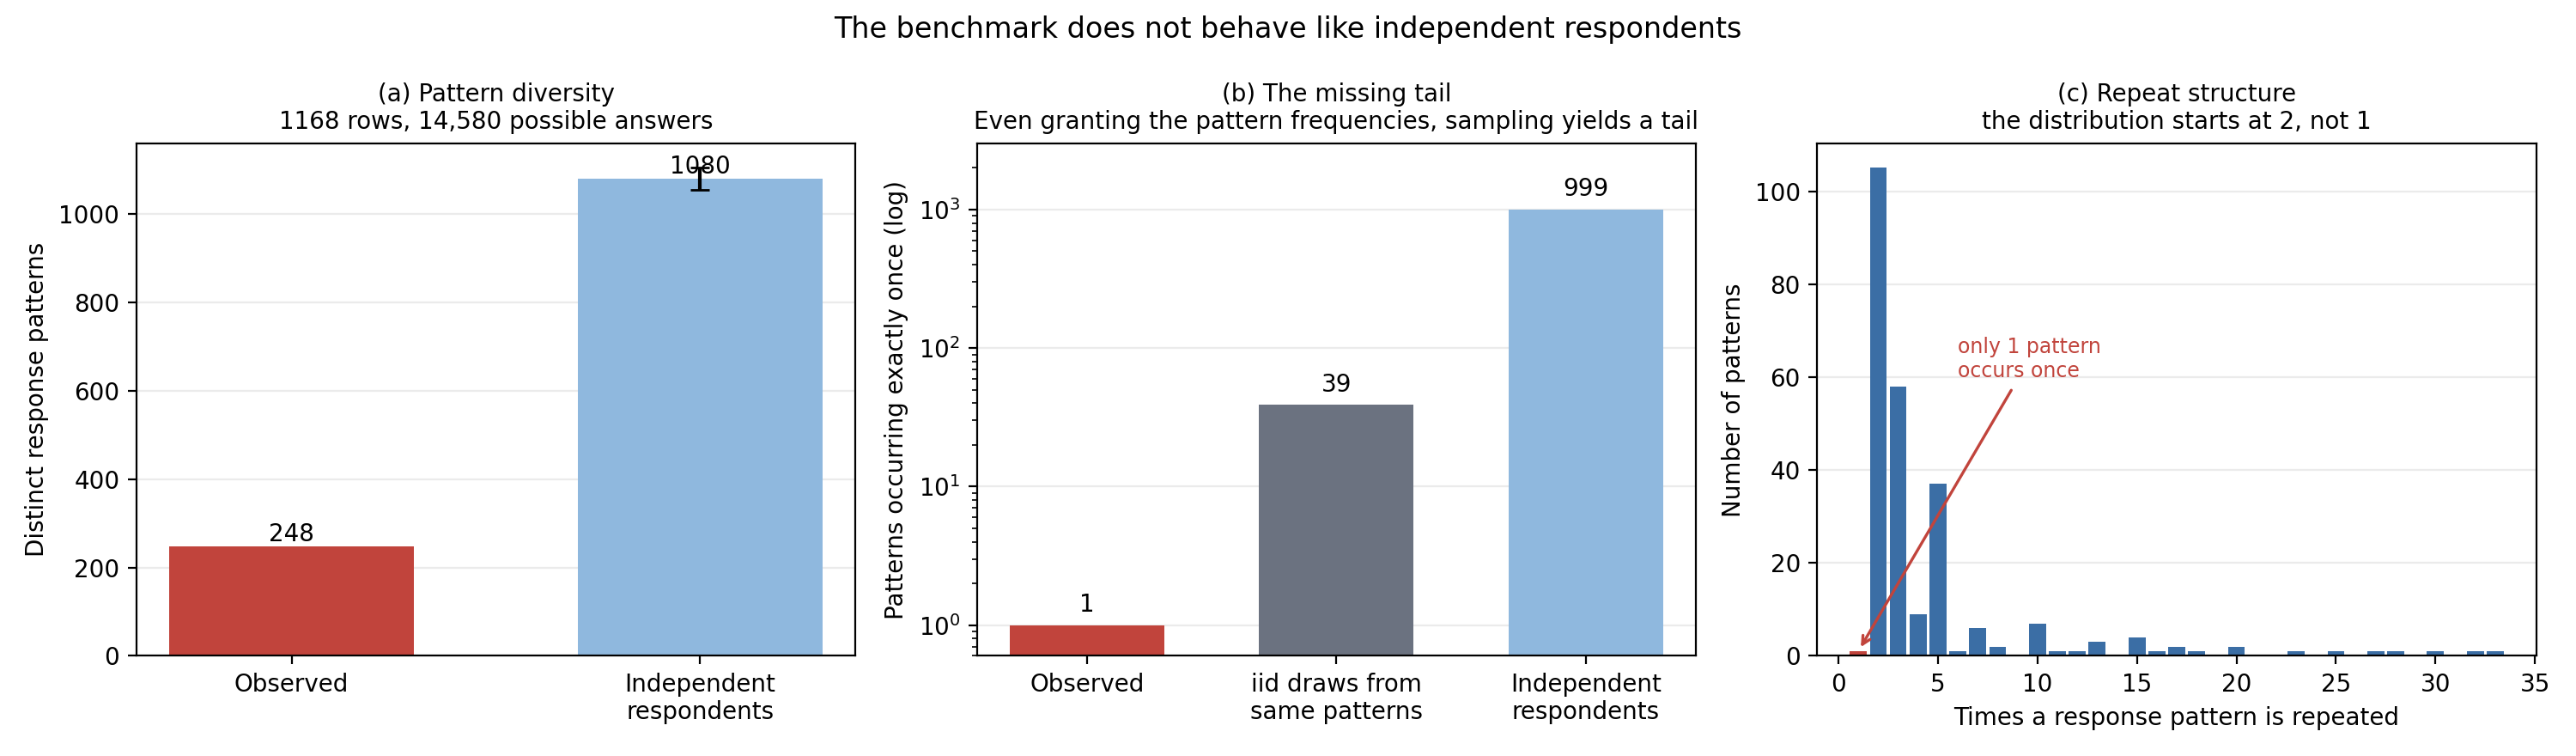
\includegraphics[width=\linewidth]{fig_audit_patterns.png}
  \caption{The benchmark does not behave like independent respondents. (a) Observed pattern
           diversity against the independence simulation. (b) Singleton patterns, log scale,
           against both nulls. (c) The empirical repeat distribution begins at two, not one.}
  \label{fig:audit:patterns}
\end{figure}

The independence simulation predicts $\approx$999 one-off patterns; the file contains
\textbf{one}. Item correlation reduces diversity and so weakens Test 1---but the observed
inter-item association is weak (Cram\'er's $V$ mostly $\approx 0.2$, maximum $0.51$), nowhere
near enough to close a gap of this size. Test 2 removes the assumption altogether and still
rejects: granting the pattern frequencies exactly, random sampling yields 39 singletons
[26--54], and the observed value of 1 lies far outside that interval. Repeat-count variance is
additionally under-dispersed relative to multinomial sampling, though only mildly
($1.2\times$); the singleton deficit, not the dispersion, is the decisive signal.

The pattern is what one expects from a limited pool of templates replicated to inflate the row
count, rather than from 1{,}503 independently sampled respondents. \textbf{The effective sample
size is the number of distinct questionnaires---248---not 1{,}503.} Every claim about
statistical power, and every model-complexity decision, should be made against that number.

\subsection{Finding 2: leakage inflation scales with model capacity}
\label{sec:audit:leakage}

Because \SI{78.8}{\percent} of rows duplicate another row, a random split places near-identical
questionnaires on both sides. We therefore evaluate every model twice under nested
cross-validation (outer 5-fold scoring, inner 3-fold grid search on ROC-AUC):

\begin{itemize}
  \item \textbf{Protocol A}---standard stratified 5-fold CV, as the literature reports.
  \item \textbf{Protocol B}---\texttt{StratifiedGroupKFold} with the group defined as the
        unique response pattern, so identical questionnaires never span a split.
\end{itemize}

\begin{figure}[htbp]
  \centering
  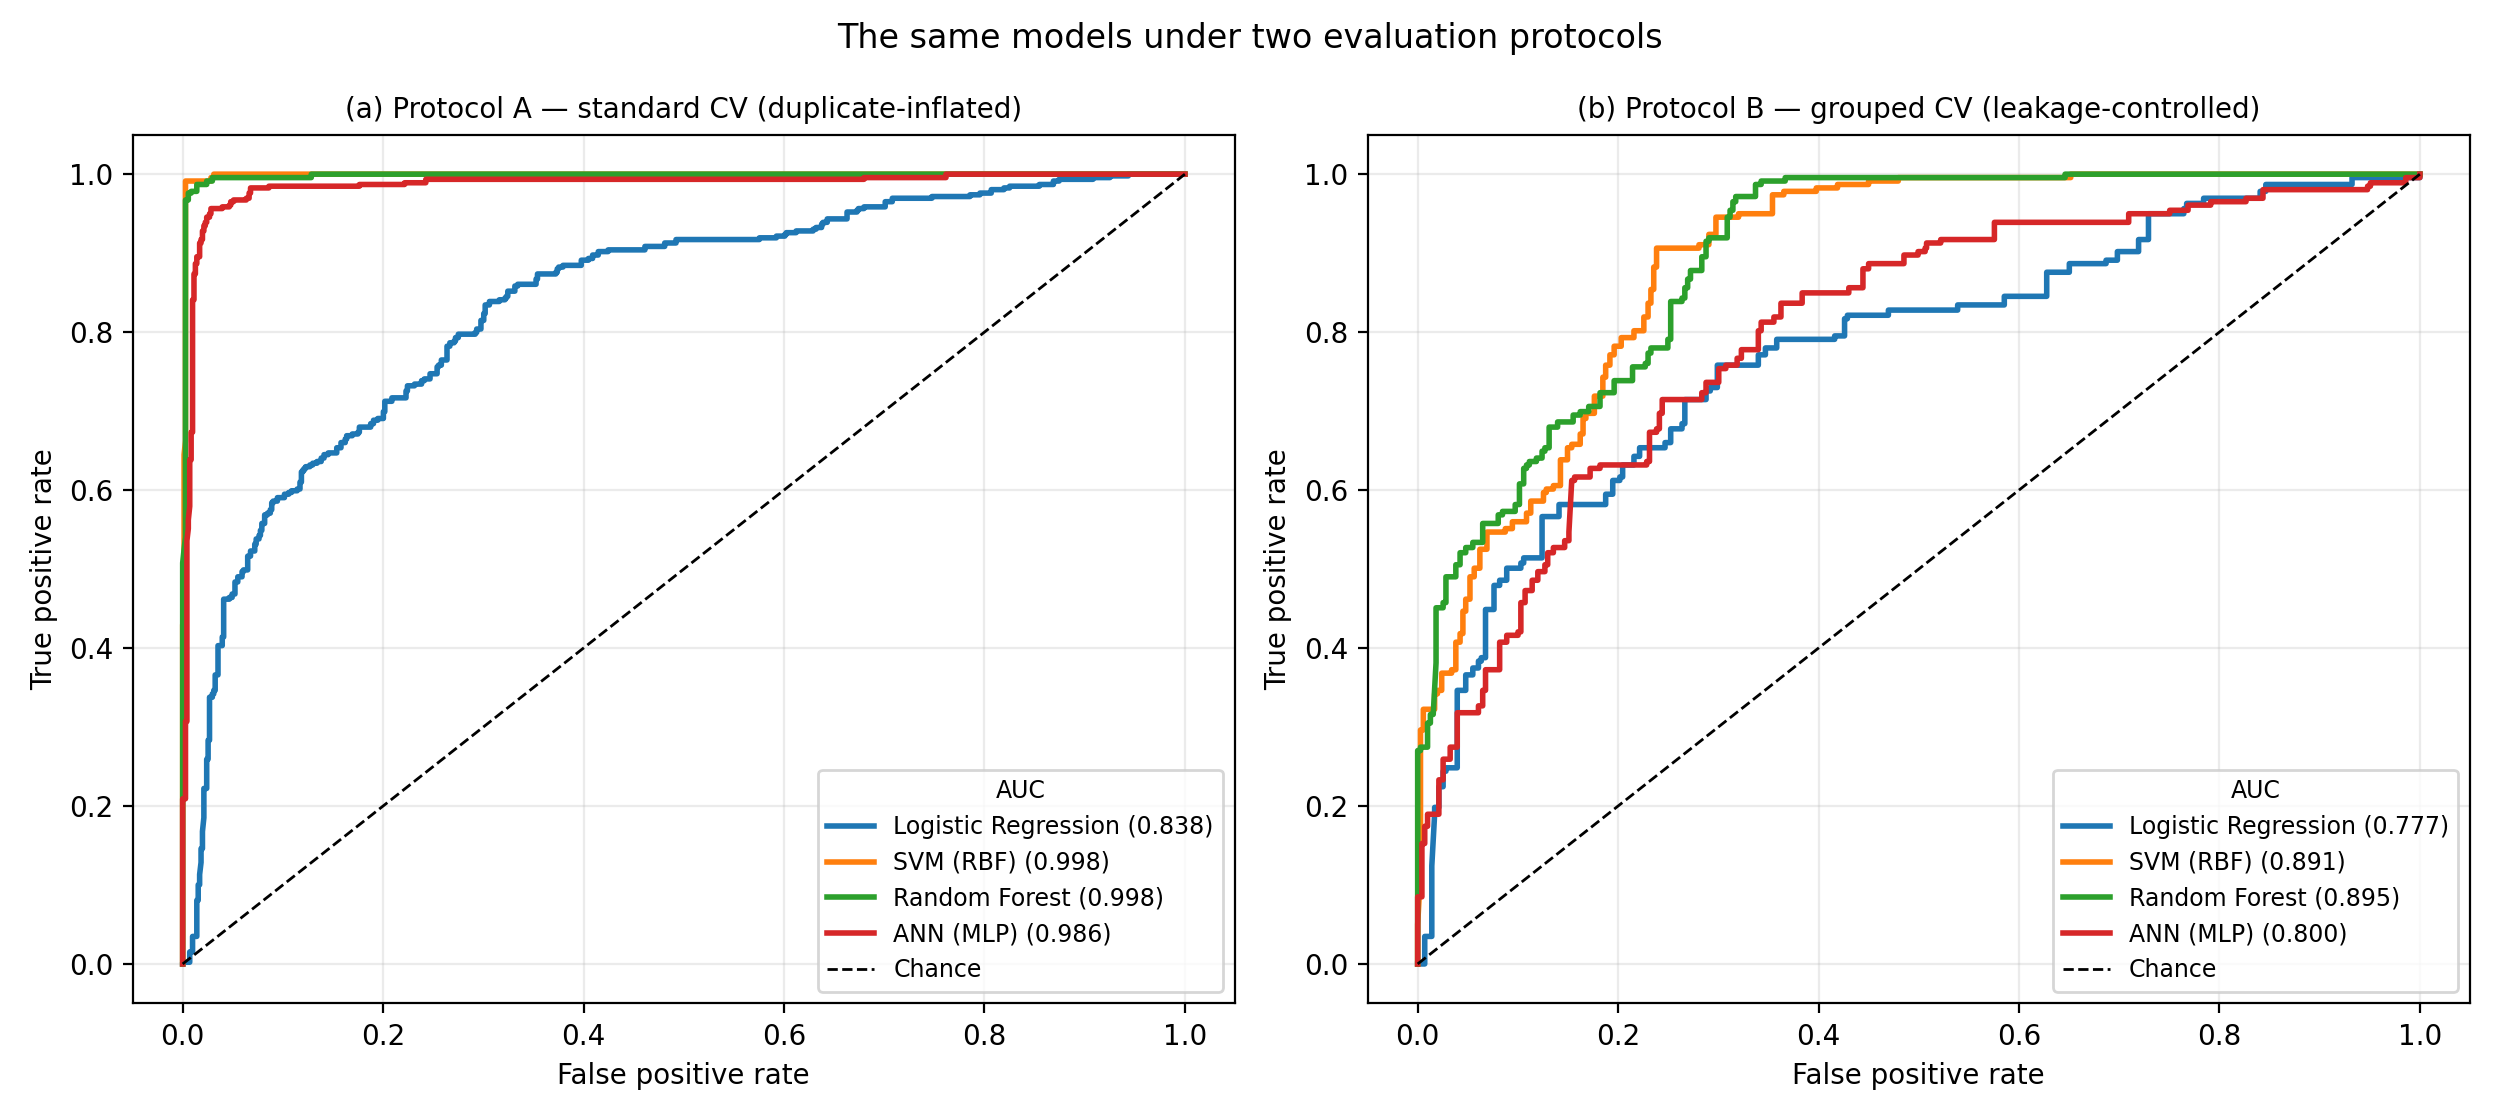
\includegraphics[width=\linewidth]{fig_audit_roc_pair.png}
  \caption{Identical models and data under the two protocols. Under Protocol A the nonlinear
           models are near-perfect; under Protocol B the same models lose most of that
           separation.}
  \label{fig:audit:roc}
\end{figure}

\begin{table}[htbp]
  \centering
  \caption{Protocol A (as reported in the literature) versus Protocol B
           (leakage-controlled). Means across outer folds.}
  \label{tab:audit:protocols}
  \begin{tabular}{lcccccc}
    \toprule
    & \multicolumn{3}{c}{Protocol A} & \multicolumn{3}{c}{Protocol B} \\
    \cmidrule(lr){2-4}\cmidrule(lr){5-7}
    Model & Acc & AUC & F1 & Acc & AUC & F1 \\
    \midrule
    Logistic Regression & 0.754 & 0.841 & 0.695 & 0.729 & 0.778 & 0.651 \\
    SVM (RBF)           & 0.991 & 0.997 & 0.989 & 0.724 & 0.891 & 0.464 \\
    Random Forest       & 0.986 & 0.998 & 0.983 & \textbf{0.784} & 0.890 & \textbf{0.714} \\
    ANN (MLP)           & 0.962 & 0.986 & 0.952 & 0.727 & 0.808 & 0.661 \\
    \bottomrule
  \end{tabular}
\end{table}

\begin{table}[htbp]
  \centering
  \caption{Inflation attributable to duplicate leakage (Protocol A $-$ Protocol B).}
  \label{tab:audit:inflation}
  \begin{tabular}{lccc}
    \toprule
    Model & $\Delta$AUC & $\Delta$F1 & $\Delta$Accuracy \\
    \midrule
    Logistic Regression & 0.063 & 0.044 & 0.025 \\
    SVM (RBF)           & 0.106 & 0.525 & 0.267 \\
    Random Forest       & 0.107 & 0.269 & 0.202 \\
    ANN (MLP)           & \textbf{0.178} & 0.291 & 0.235 \\
    \bottomrule
  \end{tabular}
\end{table}

\begin{figure}[htbp]
  \centering
  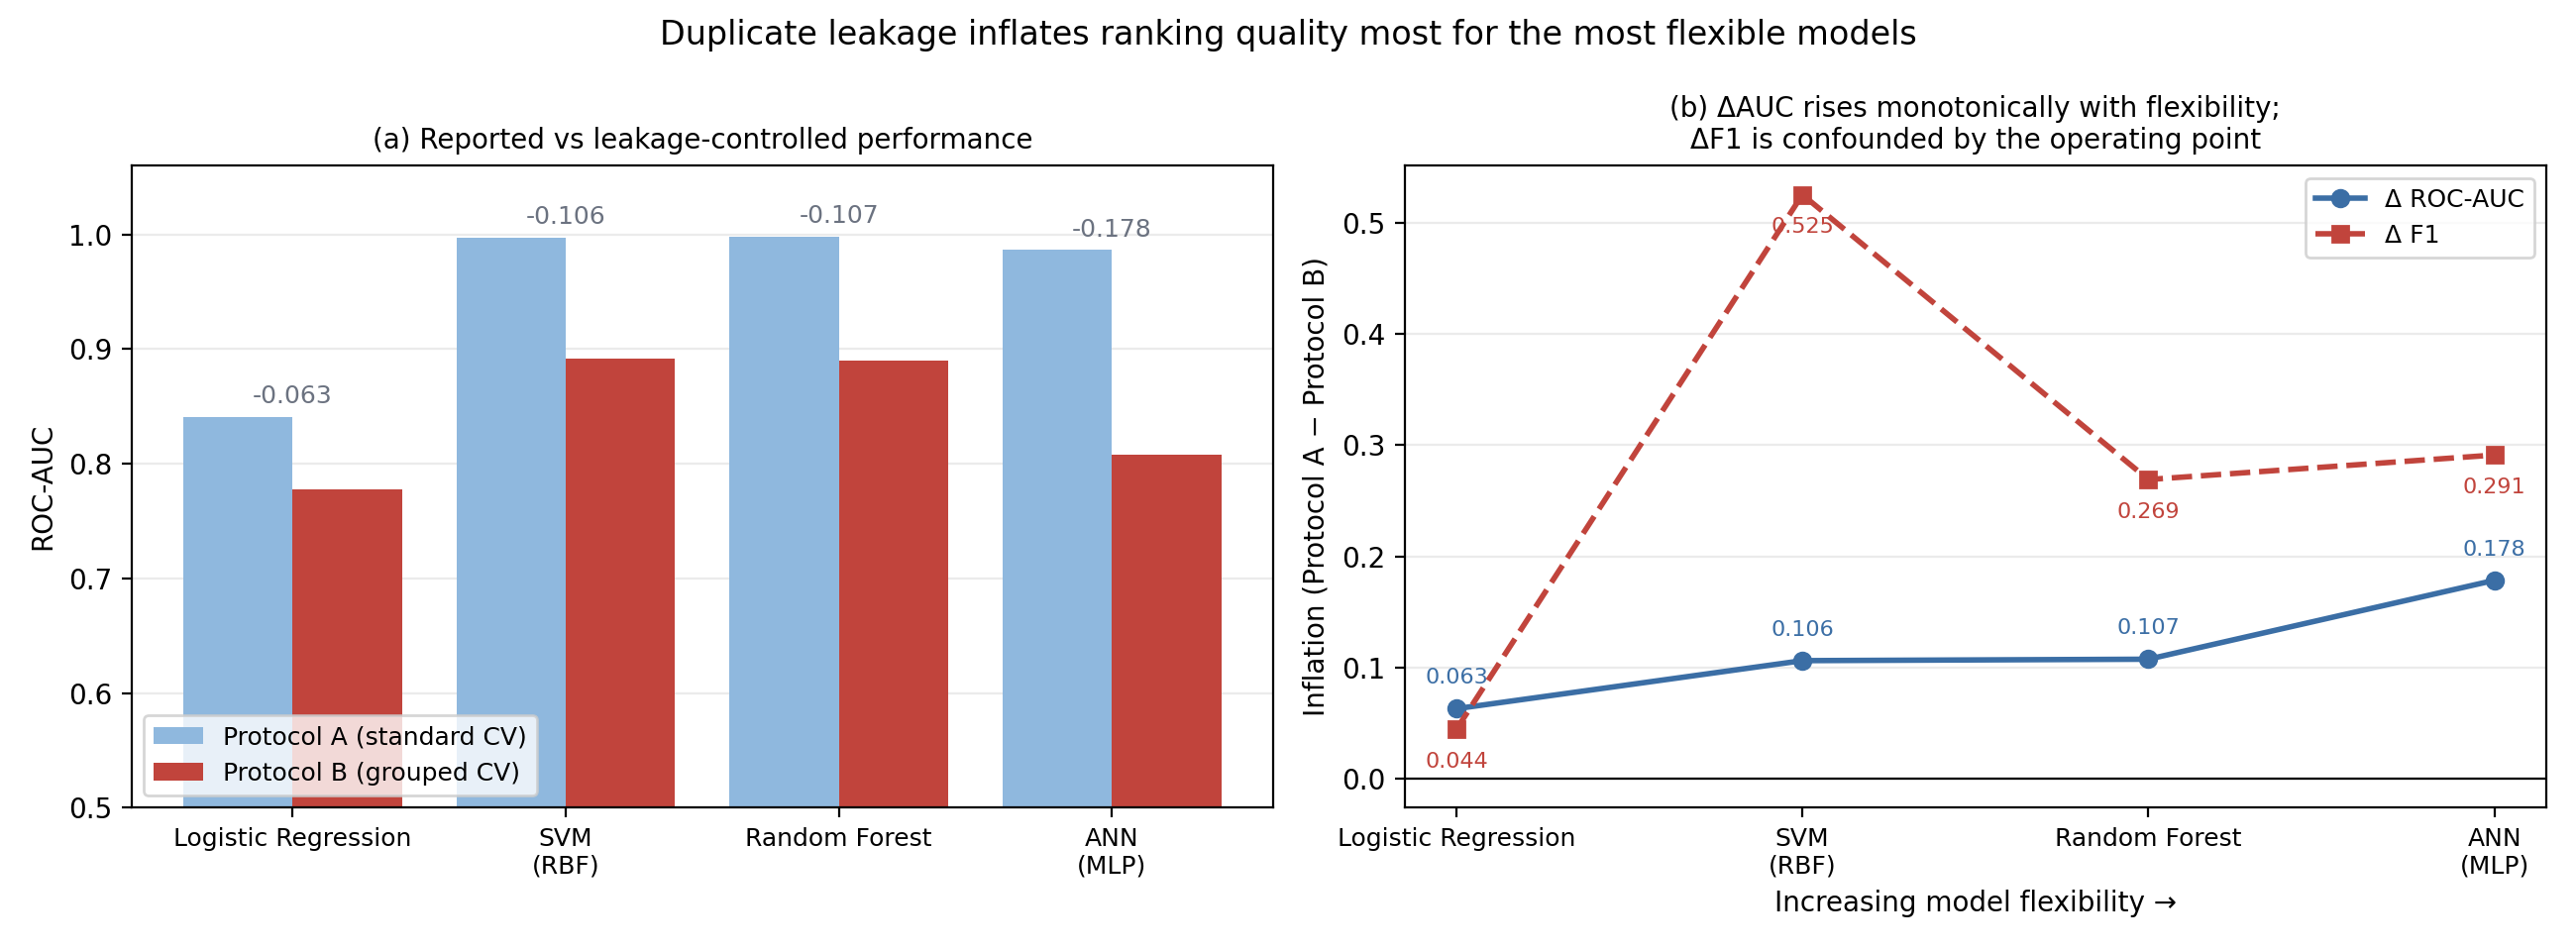
\includegraphics[width=\linewidth]{fig_audit_inflation.png}
  \caption{(a) Reported versus leakage-controlled AUC per model, annotated with the loss.
           (b) $\Delta$AUC rises monotonically with model flexibility; $\Delta$F1 is
           confounded by the operating point.}
  \label{fig:audit:inflation}
\end{figure}

\paragraph{The inflation is not uniform.} Logistic regression loses 0.063 AUC; the MLP loses
0.178, close to three times as much. Ordering models by nominal flexibility
(LR $<$ SVM-RBF $<$ RF $<$ MLP), $\Delta$AUC is monotone increasing. We do not over-read a rank
correlation computed on four points, and the SVM and Random Forest values are effectively tied
(0.106 versus 0.107); the robust statement is that the \emph{least} flexible model inflates
least and the \emph{most} flexible inflates most. The mechanism is straightforward: capacity to
memorise becomes an advantage exactly when the test set contains rows already seen.

\paragraph{The published ranking is therefore an artifact.} Under Protocol A the SVM and Random
Forest appear to dominate logistic regression by roughly 0.16 AUC---a gap that would justify
strong claims about nonlinearity in PPD risk. Under Protocol B that gap falls to
$\approx$0.11, and the SVM's F1 collapses from 0.989 to 0.464. The confusion matrices give the
sharpest view: the RBF-SVM goes from 4 false negatives to 318, missing \SI{69}{\percent} of
at-risk mothers.

We note that $\Delta$F1 is \emph{not} monotone in capacity (the SVM's 0.525 is the largest
value in Table~\ref{tab:audit:inflation}). This is a threshold artifact rather than a capacity
effect and is treated separately in \S\ref{sec:audit:threshold}; $\Delta$AUC, being
threshold-free, is the appropriate measure of the leakage effect.

\paragraph{Implication for deep learning.} At an effective $n$ of 248, capacity is a liability
rather than an asset on this branch. The MLP both inflates most under leakage and ranks
second-worst once leakage is controlled (AUC 0.808). We state this plainly because it runs
against the framing of our own architecture: the structured branch of a PPD model does not
warrant a deep network, and reported deep-learning gains on this benchmark should be treated as
unverified until reproduced under a grouped protocol.

\subsection{Finding 3: inverted symptom--risk relationships}
\label{sec:audit:validity}

Five of eight symptom items are non-monotone in severity. In four, the \emph{middle} response
level carries a lower attempt rate than reporting no symptom at all.

\begin{table}[htbp]
  \centering
  \caption{Suicide-attempt rate by response level for the four inverted items.}
  \label{tab:audit:monotonicity}
  \begin{tabular}{lccc}
    \toprule
    Item & No symptom & Middle level & Full symptom \\
    \midrule
    Feeling sad or tearful      & \textbf{0.61} & 0.20 & 0.32 \\
    Problems concentrating      & 0.45 & \textbf{0.15} & 0.62 \\
    Feeling of guilt            & 0.47 & \textbf{0.17} & 0.60 \\
    Problems bonding with baby  & 0.47 & \textbf{0.27} & 0.44 \\
    \bottomrule
  \end{tabular}
\end{table}

\begin{figure}[htbp]
  \centering
  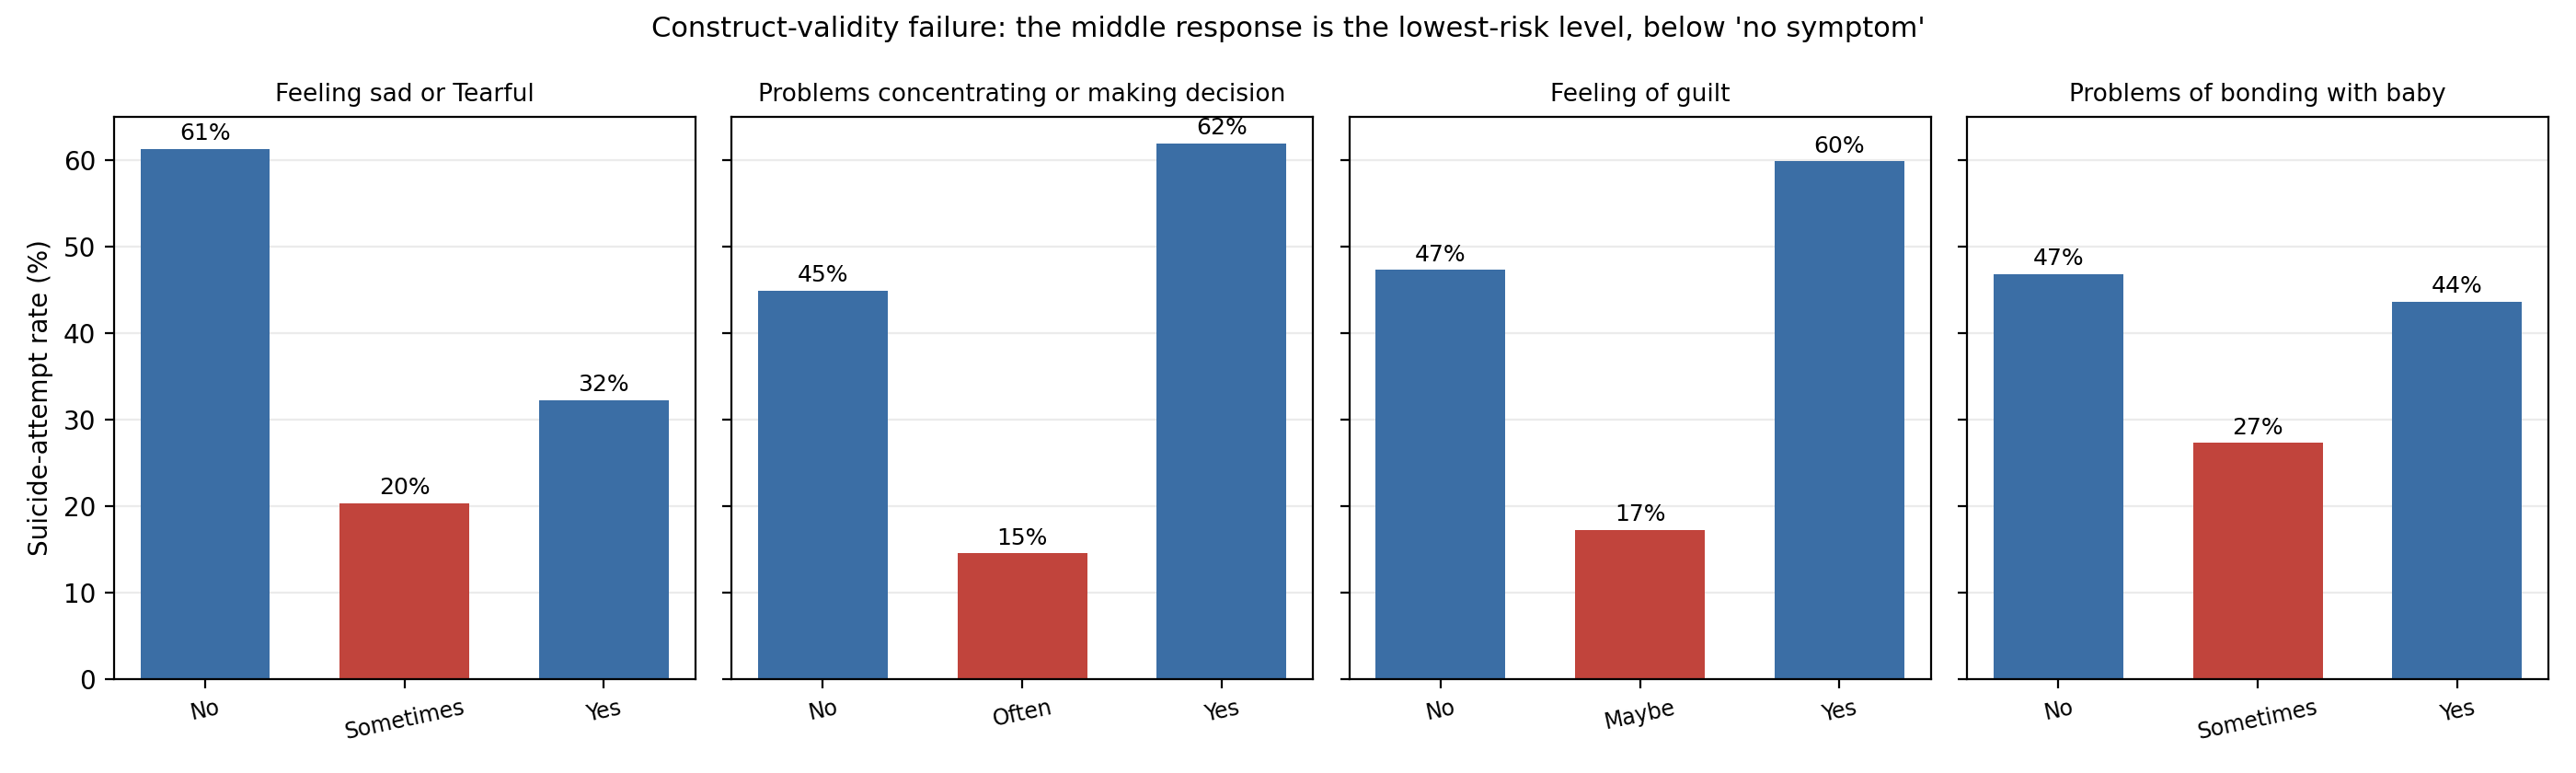
\includegraphics[width=\linewidth]{fig_audit_nonmonotone.png}
  \caption{In four items the middle response is the lowest-risk level, below ``no symptom''.}
  \label{fig:audit:nonmonotone}
\end{figure}

Respondents reporting \emph{no} sadness show a 0.61 attempt rate against 0.20 for those
reporting ``sometimes''---a threefold inversion of the clinically expected direction. A
screening instrument in which denying a symptom predicts higher risk than endorsing it
moderately is not measuring symptom severity in the intended way.

Two further items---\texttt{Feeling anxious} and \texttt{Overeating or loss of appetite}---have
no detectable association with the target ($\chi^2$ $p\approx0.73$ and $0.75$; Cram\'er's
$V=0.000$), despite anxiety being among the most robust correlates of postpartum depression in
the clinical literature.

The pattern is visible in the models too: under one-hot encoding the Random Forest ranks
\texttt{Problems concentrating = Often} and \texttt{Feeling of guilt = Maybe} as its second and
third most important features. It is also why we one-hot encode rather than treat items as
ordinal---an ordinal encoding would impose a monotonicity the data does not exhibit.

We do not claim to identify the cause. Middle-option response styles, satisficing, and
artifacts of whatever process produced the duplicate structure in \S\ref{sec:audit:n} are all
consistent with what we observe. The consequence for practice is the same either way: item
responses should not be interpreted as a severity scale.

\subsection{Finding 4: the operating point dominates model choice}
\label{sec:audit:threshold}

At the default $0.5$ threshold the RBF-SVM attains 0.971 precision with \textbf{0.307 recall},
missing 318 of 459 at-risk mothers. Selecting the threshold on training folds only (maximising
F1 within the inner CV) changes this substantially.

\begin{table}[htbp]
  \centering
  \caption{Effect of threshold selection under Protocol B. Thresholds are the mean cut-off
           chosen across outer folds.}
  \label{tab:audit:threshold}
  \begin{tabular}{lccccc}
    \toprule
    Model & Recall @ 0.5 & Recall @ tuned & F1 @ 0.5 & F1 @ tuned & Threshold \\
    \midrule
    SVM (RBF)           & 0.307 & \textbf{0.862} & 0.464 & 0.745 & 0.43 \\
    Random Forest       & 0.686 & 0.840 & 0.714 & \textbf{0.748} & 0.36 \\
    ANN (MLP)           & 0.674 & 0.749 & 0.661 & 0.675 & 0.42 \\
    Logistic Regression & 0.653 & 0.678 & 0.651 & 0.595 & 0.43 \\
    \bottomrule
  \end{tabular}
\end{table}

Moving the SVM's threshold changes recall by 0.555, while the spread in recall \emph{across all
four models} at a fixed threshold is 0.379. For a screening instrument---where a false negative
is a missed at-risk mother and a false positive is a follow-up conversation---the default
threshold is the wrong operating point, and accuracy at that threshold is the wrong headline
metric. We recommend that screening work on this task report decision-curve or net-benefit
analysis at explicit cost ratios instead.

\subsection{Recommended protocol and corrected baselines}
\label{sec:audit:protocol}

For survey-derived mental-health datasets we recommend that evaluation \textbf{group on the
unique feature pattern}, not on the row: hash the feature vector, use it as the group key in
\texttt{StratifiedGroupKFold}, and report the resulting scores as primary. Where comparison
with prior work is needed, report the standard-split figure alongside and label it as such.

The corrected reference baselines are the Protocol B columns of
Table~\ref{tab:audit:protocols}. The honest ceiling is $\approx$0.89 AUC and $\approx$0.75 F1,
attained by the Random Forest at a tuned threshold---not the $\approx$\SI{99}{\percent}
accuracy widely reported. We recommend this dataset be treated as an \textbf{audit object
rather than as training data}; work requiring a genuine structured branch should use a
population survey with clinical labels (e.g.\ PRAMS) or an EPDS-labelled cohort.

\subsection{Implication for the multimodal architecture}
\label{sec:audit:implication}

This audit changes the empirical footing of the multimodal design rather than undermining it.
The structured branch's honest ceiling ($\approx$0.89 AUC / $\approx$0.75 F1) is measured on a
\emph{concurrent} severity proxy: the target is co-reported with the symptoms used to predict
it, within a single questionnaire. That is screening, not anticipation. The claim that a
structured symptom inventory is insufficient for anticipatory PPD detection therefore moves
from a motivating assertion to a measured result, and Protocol B supplies the floor that any
text or multimodal branch must clear to justify its complexity.

\subsection{Limitations}
\label{sec:audit:limitations}

\begin{itemize}
  \item \texttt{Suicide attempt} is a self-reported severity proxy, not a clinical diagnosis,
        and is predicted from symptoms co-reported in the same instrument.
  \item Test 1 in \S\ref{sec:audit:n} assumes inter-item independence and therefore overstates
        expected diversity. Test 2 does not rely on that assumption and is the claim we rest on.
  \item We characterise the duplicate structure as inconsistent with independent sampling. We
        do not have provenance information for the file and do not assert \emph{how} it was
        produced.
  \item The capacity ordering in \S\ref{sec:audit:leakage} is nominal; with four models we
        report the endpoints rather than a rank statistic.
  \item The threshold analysis in \S\ref{sec:audit:threshold} optimises F1; a deployment would
        select the operating point against an explicit clinical cost ratio.
\end{itemize}
